\chapter{Monitorowanie procesu gojenia ścięgna Achillesa}
\section{Ścięgno Achillesa}
Ścięgno Achillesa, nazywane również ścięgnem piętowym, jest największym i najsilniejszym ścięgnem występującym w ciele ludzkim. Stanowi wspólne zakończenie mięśnia trójgłowego łydki, w którego skład wchodzą dwie głowy mięśnia brzuchatego i mięsień płaszczkowaty. Całość struktury zlokalizowana jest w tylnym, powierzchownym przedziale łydki, co zostało przedstawione na Rysunku \ref{muscle_structure}.  
\begin{figure}[h!]
\centering
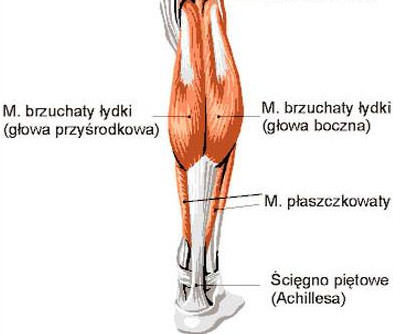
\includegraphics[width=0.55\textwidth]{figures/muscleStructure.jpg}
\caption{Lokalizacja mięśnia trójgłowego łydki wraz ze ścięgnem Achillesa.}
\label{muscle_structure}
\end{figure}
Z obu głów (brzuścców) mięśnia brzuchatego łydki wyrasta jedno szerokie, płaskie ścięgno, które jest początkiem części brzuchatej ścięgna Achillesa. Następnie ścięgno to łączy się z włóknami pochodzącymi od mięśnia płaszczkowatego, które układają się stycznie do wcześniej powstałej struktury. Wówczas kształt ulega stopniowemu zwężeniu i zaokrągleniu, aż do punktu o minimalnej szerokości (około 4 cm nad przyczepem dolnym [1]). W rejonie samego przyczepu dolnego znajdującego się na tylnej powierzchnia kości piętowej, ścięgno ponownie jest płaskie i szerokie.

W kolejnych podsekcjach szczegółowo omówiona została anatomia ścięgna Achillesa, jego biomechanika, potencjalne urazy wraz z czynnikami im sprzyjającymi oraz proces gojenia i możliwości jego wspomagania. Wszystkie te aspekty są istotne z uwagi na możliwości monitorowania procesów fizjologicznych występujących w ścięgnie. 
\subsection{Anatomia}
Średnia długość ścięgna Achillesa to 15 cm (11 - 26 cm). Średnia szerokość w rejonie początku wynosi 6.8 cm (4,5 - 8, 6 cm). Następnie, stopniowo ścięgno ulega zwężeniu do punktu o minimalnej szerokości 1.8 cm (1,2 - 2,6 cm). W rejonie samego przyczepu struktura ponownie się rozszerza i jej szerokość wynosi średnio 3.4 cm (2,0 - 4,8 cm) [2-3].
Zewnętrzną część ścięgna Achillesa stanowi ościęgno utworzone z tkanki łącznej włóknistej.
Achil
-Histologia
-Unaczynienie (krew, nerwy)

\subsection{Biomechanika}
Zadaniem ścięgien jest transfer siły mięśniowej do układu szkieletowego.
\subsection{Urazy i czynniki im sprzyjające}
\subsection{Leczenie, fazy gojenia i rehabilitacja}
\section{Zastosowanie rezonansu magnetycznego}
\section{Zastosowanie ultrasonografii}

Kolejną z metod obrazowania medycznego jest \textit{Ultrasonografia}, w skr. \textit{USG} (ang. \textit{Ultrasonography}, \textit{US}). Bazuje ona na efektach związanych z propagacją w tkankach \textit{ultradźwięków}, tj. fal akustycznych o częstotliwościach powyżej 20 kHz.

Propagacja fal w przyrodzie była tematem rozważań myślicieli takich jak Pitagoras, Arystoteles czy Galileusz, którzy ugruntowali pole badań pod kolejne osiągnięcia matematyczno-inżynieryjne. W tej kwestii, do jednego z przełomów doszło w 1822 roku, kiedy to szwajcarski inżynier Daniel Colladen oraz matematyk Charles-Francois Sturm wyznaczyli przybliżoną prędkość rozchodzenia się fali akustycznej w wodzie. Badanie wykonano na Jeziorze Genewskim, symultanicznie mierząc czas jaki potrzebny był dźwiękowi podwodnego wystrzału i sygnałowi dzwonka rozchodzącego się w powietrzu, aby przebyły drogę pomiędzy dwoma łódkami oddalonymi o 10 mil. Wyliczona wartość wyniosła wówczas 1435 m/s, nie różniąc się znacząco od dzisiaj przyjmowanej estymacji równej 1484 m/s. 

58 lat później, w 1880 roku bracia Curie opisali w \cite{Curie1880} \textit{efekt piezoelektryczny}, czyli zjawisko polegające na pojawieniu się ładunku elektrycznego pod wpływem naprężeń mechanicznych w krysztale o anizotropowej budowie, takiej jak ma np. kwarc. W przypadku odwrotnym, przyłożenie napięcia do odpowiedniego kryształu generuje drgania. Efekty te są wykorzystywane w \textit{głowicy aparatu usg}, przyrządu do generowania i odbierania ultradźwięków. 

Przykładowo polaryzowanie kryształu piezoelektrycznego krótkim impulsem typu $\sigma(t)$ pobudza go do drgań gasnących na własnej częstotliwości rezonansowej. Jeżeli kryształ piezoelektryczny ma kształt walca o grubości $x$=0,64mm, to będzie stanowił rezonator półfalowy, w którym wystąpi drganie rezonansowe o długości fali $\lambda = 2x$ czyli $\lambda = 1,28$ mm. Jeżeli wykonany jest z tytanianu baru, dla którego prędkość propagacji drgań wynosi $c$=4460m/s, to częstotliwość drgań własnych tego
kryształu wyniesie:
\begin{equation}
f = \frac{c}{\lambda} = \frac{4460 m/s}{1,28 mm} = 3,5 MHz
\end{equation}

Fale generowane przez głowicę aparatu USG rozchodzą się w tkankach miękkich i podobnie jak w doświadczeniu Colladena, można ocenić czas pomiędzy nadaniem i odbiorem sygnału. Dodatkowo we współczesnych aparatach pomiarowych analizowana jest również różnica w amplitudzie i częstotliwości fali nadawanej i odbieranej. Zmiany te są efektem zróżnicowania \textit{impedancji akustycznej ośrodka} $Z$ wyrażanej jako:
\begin{equation}
Z = \rho c = \sqrt{\epsilon \rho},
\end{equation}
gdzie $c$, to prędkość rozchodzenia się fali, $\rho$ to gęstość ośrodka, a $\epsilon$ to \textit{moduł odkształcalności objętościowej}, tj. parametr opisujący jak zmieni się objętość ośrodka pod danym ciśnieniem. Parametry wybranych ośrodków zestawiono w Tabeli \ref{USG-params} 
\begin{figure}[h!]
	\centering
	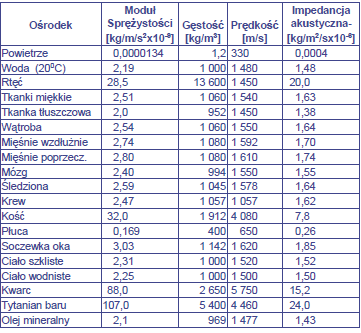
\includegraphics[width=0.55\textwidth]{figures/USG-params.png}
	\caption{Parametry ośrodków często mierzonych w badaniach USG.}
	\label{USG-params}
\end{figure}
Kiedy fala pada na granice dwóch ośrodków o różnych impedancjach akustycznych $Z_1$ i $Z_2$ dochodzi do zjawiska częściowego bądź całkowitego odbicia opisanego prawem Snella:
\begin{equation}
R = \frac{I_r}{I_0} = \left(\frac{Z_1-Z_2}{Z_1+Z_2}\right)^2,
\end{equation}
gdzie $I_0$ to natężenie fali padającej, a $I_0$ odbitej. Natomiast $R$, czyli współczynnik odbicia rośnie wraz ze wzrostem kąta odchylenia od kierunku prostopadłego, aż do całkowitego odbicia.

Fala propagująca się w ośrodku ulega również osłabieniu w wyniku różnego rodzaju efektów związanych z absorpcją i rozpraszaniem energii, co zapisywane jest następująco:
\begin{equation}
I=I_0 \epsilon^{-\gamma x},
\end{equation}
gdzie $\gamma$ to współczynnik osłabienia, a $x$ to droga przebyta przez falę. Korekcję osłabiania fali w zadanym torze propagacji fali wykonuje się najczęściej manualnie poprzez dobór odpowiedniego natężenia fali wytwarzanej w głowicy USG, tj. w praktyce takiego, który umożliwi radiologowi możliwie najlepszą obserwacje danego ośrodka. 

Dodatkowo należy zwrócić uwagę, że każdy punkt powierzchni drgającego przetwornika jest źródłem fali kulistej, emitowanej w ośrodku nagłaśnianym. W pobliżu przetwornika występują z tego powodu liczne interferencje, zarówno poprzeczne jak i wzdłużne. Obszar, w którym interferencje występują, nazywany jest \textit{polem bliskim}. Obszar, w którym fala mechaniczna propaguje się już w sposób jednorodny, bez interferencji, nazywany jest polem dalekim. 

/*o dopplerze masz więcej w beamforming.pdf*/
W przypadku przechodzenia fali przez ośrodki względem siebie się przesuwające dochodzi do efektu Dopplera zapisywanego wzorem:
\begin{equation}
F = 2 f_o\frac{v}{c}(v/c)\cos{Q},
\end{equation} 
gdzie $F$ to zmiana częstotliwości fali nadawanej $f_0$, zależna od kąta $Q$ pomiędzy falą i ośrodkiem poruszającym się i prędkościami rozchodzenia się fali w obu ośrodkach tj. $v$ i $c$. Efekt Dopplera jest wykorzystywany w praktyce np. do monitorowania przepływu krwi w tkankach.

Podsumowując, obecnie stosowana najczęściej rekonstrukcja obrazu USG (tzw. \textit{beamforming}) wygląda następująco:

/*zamień poniższy tekst na punkty*/

Obraz tworzony jest w ten sposób, że głowica ultradźwiękowa emituje impulsy w
postaci wąskiej wiązki w ściśle określonym kierunku. Wiązka zawiera sygnał z $N$ przetworników składających się z kryształów piezoelektrycznych\footnote{nowością i przewidywaną przyszłością USG jest praktyczne stosowanie przetworników w technologii cMUT i pMUT, co umożliwia miniaturyzację urządzeń np. [http://news.mit.edu/2018/startup-butterfly-network-ultrasound-smartphone-0207]} 

Następnie odbiera z tego kierunku echa, powstające na niejednorodnościach struktur biologicznych. Wypadkowa charakterystyka kierunkowa jest iloczynem charakterystyk przy nadawaniu i odbiorze, co pozwala na formowanie pojedynczego promienia akustycznego. Po odsłuchaniu i zapamiętaniu wszystkich ech z tego promienia
głowica ultradźwiękowa emituje kolejny promień. Po zapamiętaniu ech ze wszystkich
promieni, a we współczesnych aparatach USG jest ich od 32 do 512, aparat wyświetla zapamiętany obraz. Obraz I może być tworzony we współrzędnych biegunowych – głowice: mechaniczna sektorowa,
I(r,$\theta$) wieloelementowa convex, fazowa.
We współrzędnych prostokątnych – głowice: mechaniczna liniowa,
I(x,y) wieloelementowa liniowa. Niewielka prędkość propagacji ultradźwięków w tkance powoduje, że obraz w
prezentacji I jest obrazem stacjonarnym. Jeżeli na obraz I składa się 400 promieni i
każdy odsłuchiwany jest do głębokości 25cm, to czas gromadzenia danych wynosi
2x25cm/1500m/sx400 = 0,133s. Daje to około 8obrazów/s. Poprawa stosunku
31
sygnał-szum, uzyskiwana metodą uśredniania kilku kolejnych obrazów prowadzi do
dalszego wydłużenia czasu gromadzenia obrazu – do około 0,5s lub więcej (nawet
do 2s). 

Do najważniejszych zalet USG należy zaliczyć:
\begin{itemize}
	\item możliwe obrazowanie w czasie rzeczywistym.
	\item pomiary morfologiczne i fizjologiczne.
	\item niskie koszty w porównaniu np. do MR czy TK.
	\item bezpieczeństwo - promieniowanie jest niejonizujące jak w przypadku promieni Rentgena.
\end{itemize}

/*Kontekst ścięgna wykorzystujący te plusy:
W kontekście monitorowania gojenia się ścięgna zwraca się uwagę na unaczynienie tkanek miękkich, które być szczególnie intensywne w 1 fazie gojenia się ścięgna i stopniowo zanikać w kolejnych okresach.

Funkcjonalne i morfologiczne i doppler
*/

\section{Zastosowanie badań biomechanicznych}
\section{Inne metody}